\chapter{Construction d'une architecture modulaire de cartes auto-organisatrices}
Le but de cette thèse est de proposer les bases d'un modèles permettant d'associer des cartes auto-organisatrices dans un cadre général. 


\section{Description de l'algorithme}

\begin{figure}
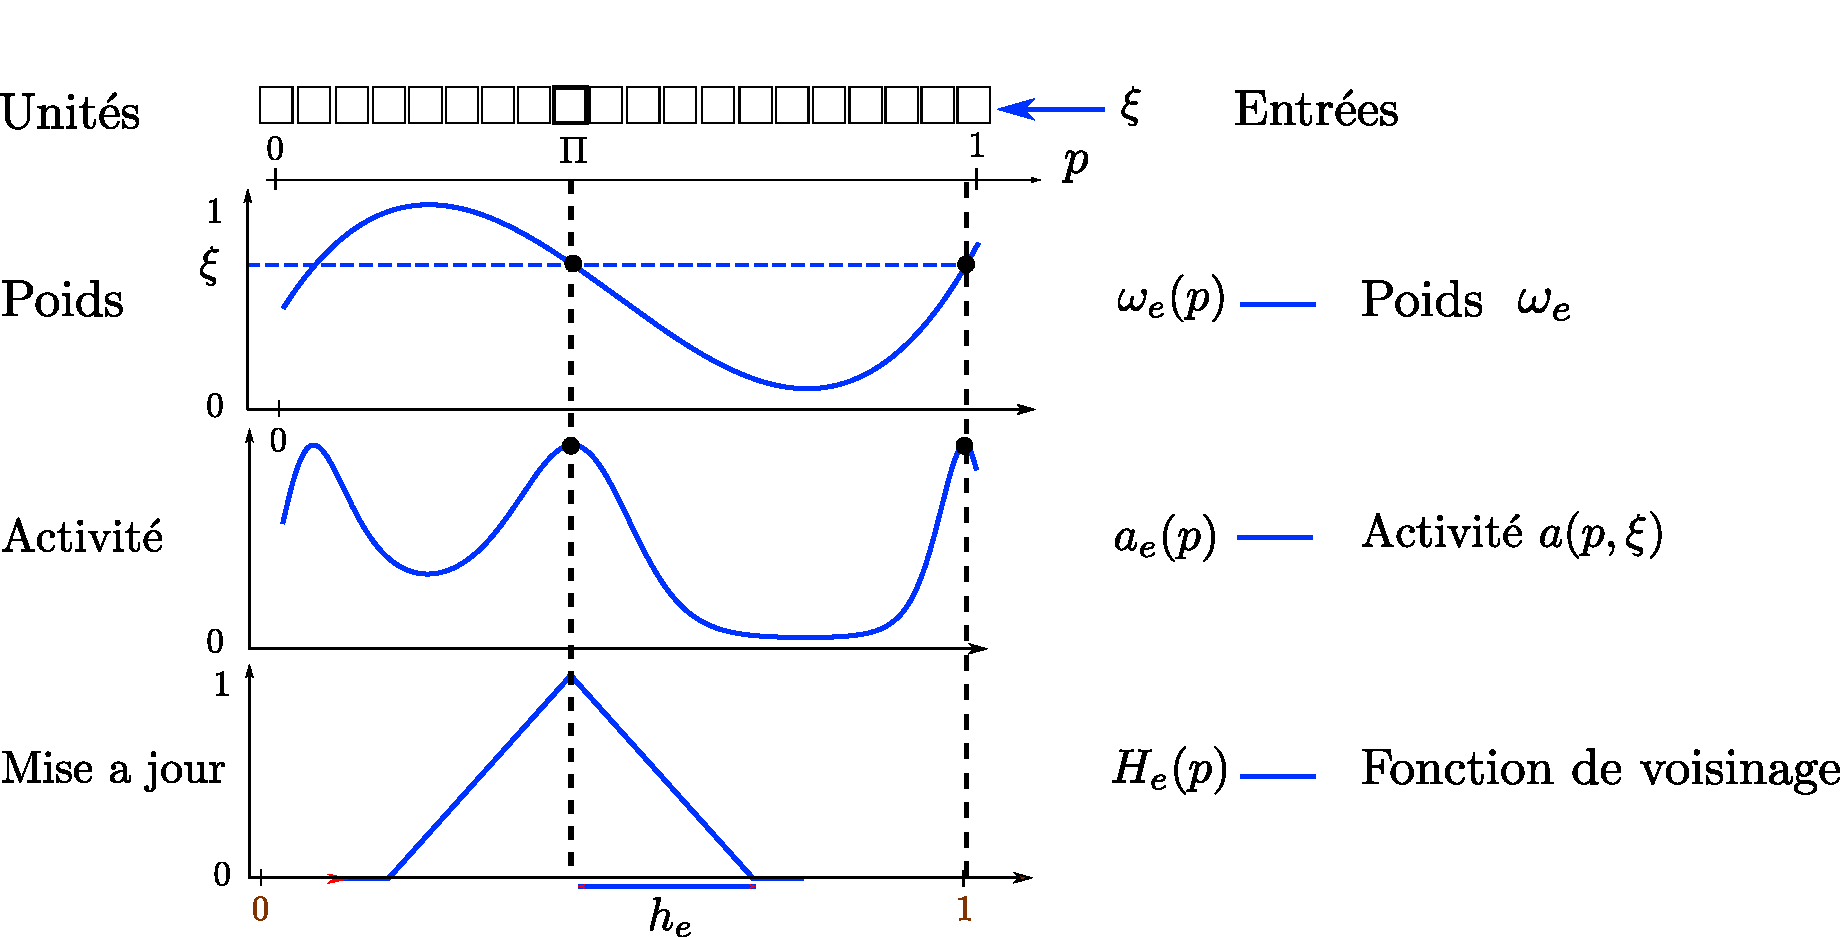
\includegraphics[width=\textwidth]{one_map_one_layer.pdf}
\caption{Notation utilisées dans une carte de Kohonen en 1 dimension}
\label{fig:one_map_not}
\end{figure}


\begin{figure}
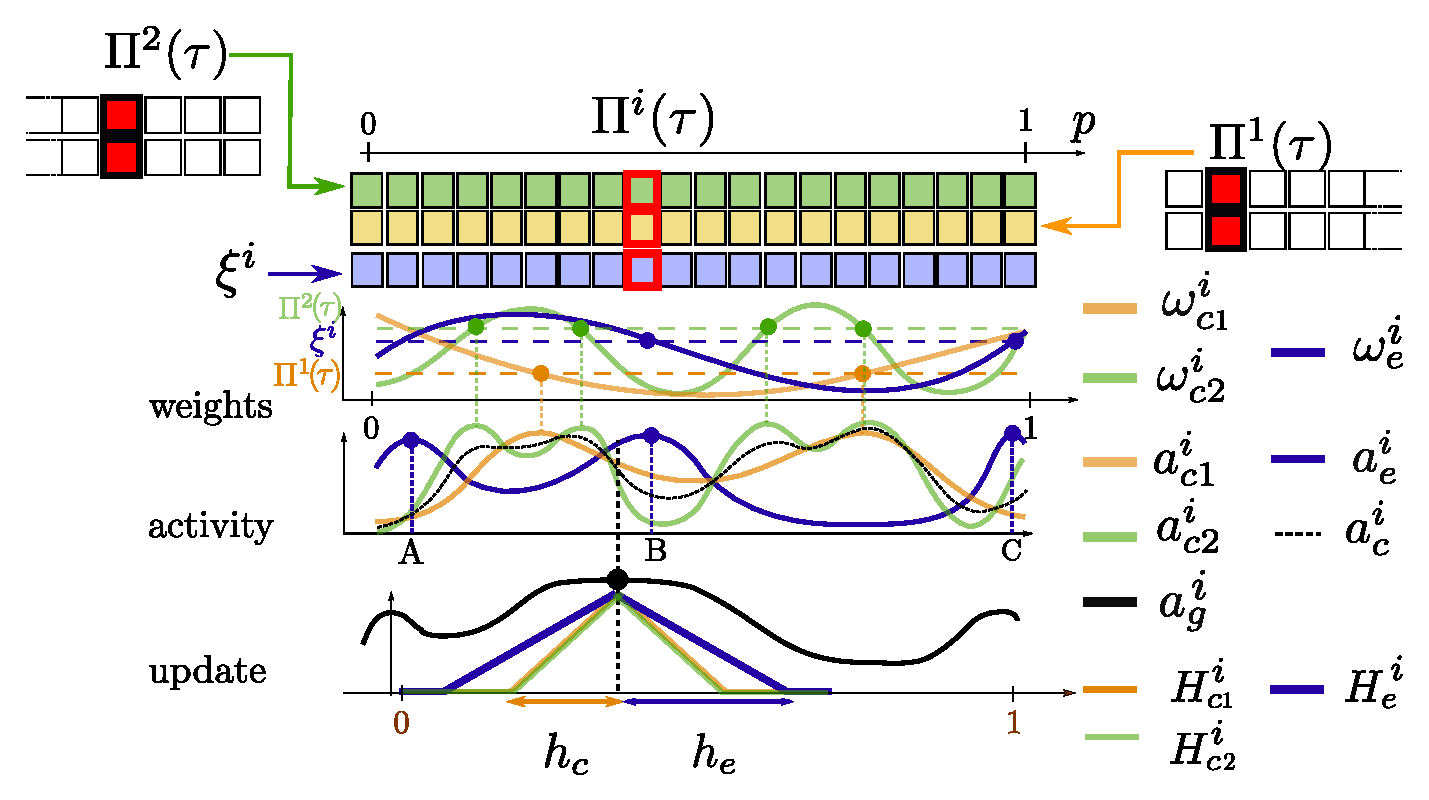
\includegraphics[width=\textwidth]{one_map.pdf}
\caption{Description d'une carte au sein d'une architecture CxSOM, avec une seule connexion.}
\label{fig:one_map}
\end{figure}


\section{Choix des paramètres}

\subsection{Influence des rayons de voisinage}

\subsection{Influence des autres paramètres}

\subsection{Compatibilité en 2D}

\section{Analyse de la relaxation}

L'apprentissage conjoint des cartes repose sur la relaxation au sein d'une itération. On cherche donc à vérifier si la relaxation converge vers une valeur quelle que soit l'entrée, et si elle est pertinente en large dimension avec de nombreuses cartes.

\subsection{Analyse expérimentale}

\subsection{Champs de BMU}

\subsection{Limitations et possibilités en grande dimension}

\section{Implémentation}
L'histoire de la recherche de consensus dans le graphe de cartes, permet que ce soit vraiment décentralisé